\documentclass[a0,final, portrait]{inriaposter}

\usepackage[utf8]{inputenc}
\usepackage[OT1]{fontenc}
\usepackage[english]{babel}
\usepackage{amsfonts, amsmath, amssymb, amsthm, dsfont, amsthm}
\usepackage{paralist}
\usepackage{wrapfig}

\usepackage{caption}
\usepackage{subcaption}

\usepackage{graphics}
\usepackage{graphicx}

\usepackage{epstopdf}

\providecommand{\mtx}[1]{\mathbf{#1}}

\begin{document}

\sffamily

\postertitle%
{A new experimental setup \\ to study the structure of curiosity-driven exploration in humans}
{Brice Miard \textsuperscript{1} and Pierre Rouanet \textsuperscript{1}, Jonathan Grizou \textsuperscript{1}, \\
Manuel Lopes \textsuperscript{1}, Jacqueline Gottlieb \textsuperscript{2}, Adrien Baranes \textsuperscript{2}, Pierre-Yves Oudeyer \textsuperscript{1}}
{\Large  \textsuperscript{1} Flowers Team,  INRIA / ENSTA ParisTech, France \; --- \; \textsuperscript{2} Department of Neuroscience, Columbia University}


\vfill
\Large
\begin{multicols}{2}

\blockabstract{
Curiosity is a key element of human development, driving us to explore spontaneously novel objects, activities and environments~\cite{gottlieb2013information}. Curiosity-driven exploration strategies permit us to interact, learn and evolve quickly in an open ended world. It is thus an important challenge to understand the fundamental mechanisms of spontaneous exploration and curiosity in humans.

~~~~~Novel hypotheseses have been formulated such that curiosity-driven sensorimotor exploration could be organized as to maximize learning progress \cite{oudeyer2007intrinsic}, which is different from more classical hypothesis conceptualizing curiosity as a drive to maximize uncertainty of novelty. Yet, experimental setups designed so far in the literature do not allow to separate between these hypotheses.

~~~~~We make a step in this direction by presenting an exploratory study with humans designed to analyze and measure properties of curiosity-driven exploration of a priori unknown sensorimotor spaces. More specifically, we are interested in the relation between exploration and learning progress.

}

\block{Experimental Setup}{


\begin{center}
    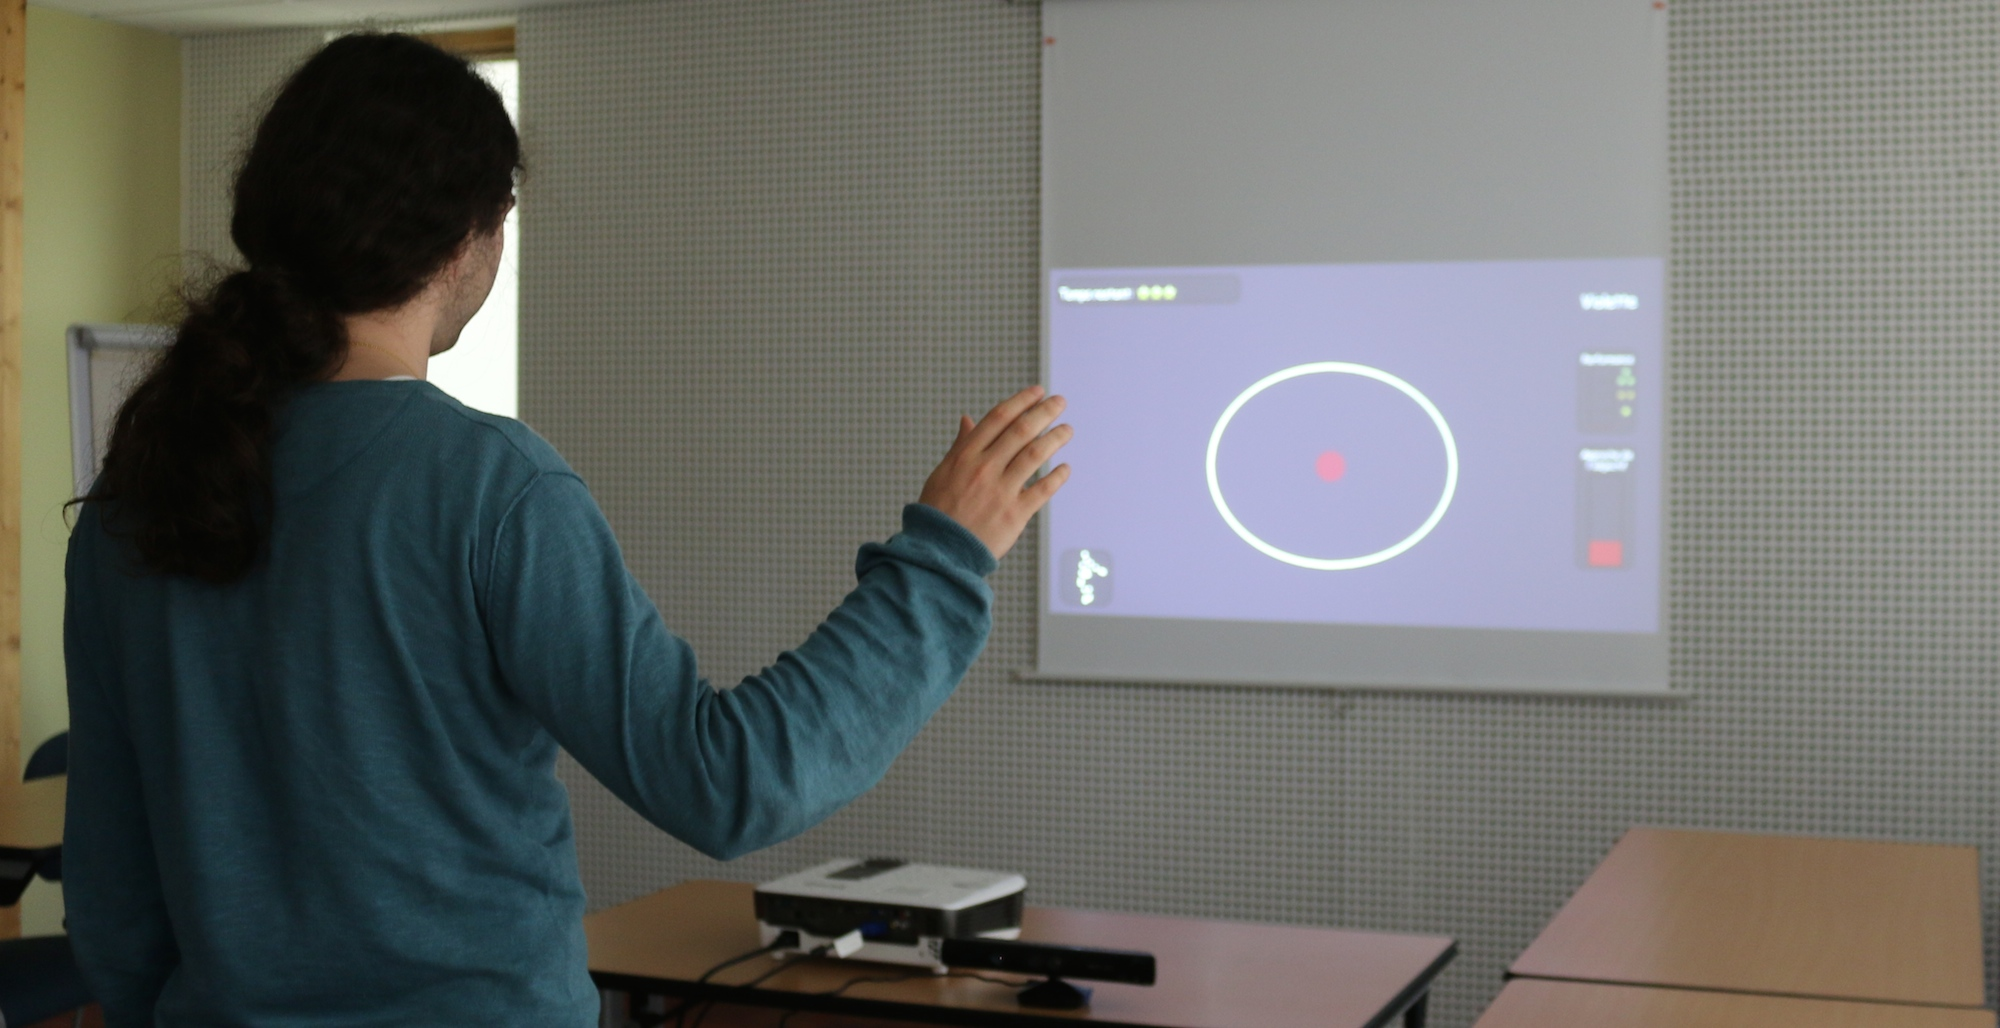
\includegraphics[width=0.9\columnwidth]{images/setup-1.JPG}
\end{center}

{\large Photo of the experimental setup. A kinect sensor is used to capture the body motion of the subject that is mapped to a two-dimensional shape on the screen. The goal of the participant is to control the shape to match a specific goal shape.}

\vspace{2cm}

While users were extrinsically motivated to play each game (protocol, score...), they coul freely switch from one game to another (among four similar games) whenever and as many times as they wanted during the 15 minutes the experiment lasted. While all games have a similar structure, each game has a different mapping and thus a different complexity.

\vspace{2cm}

\begin{center}
    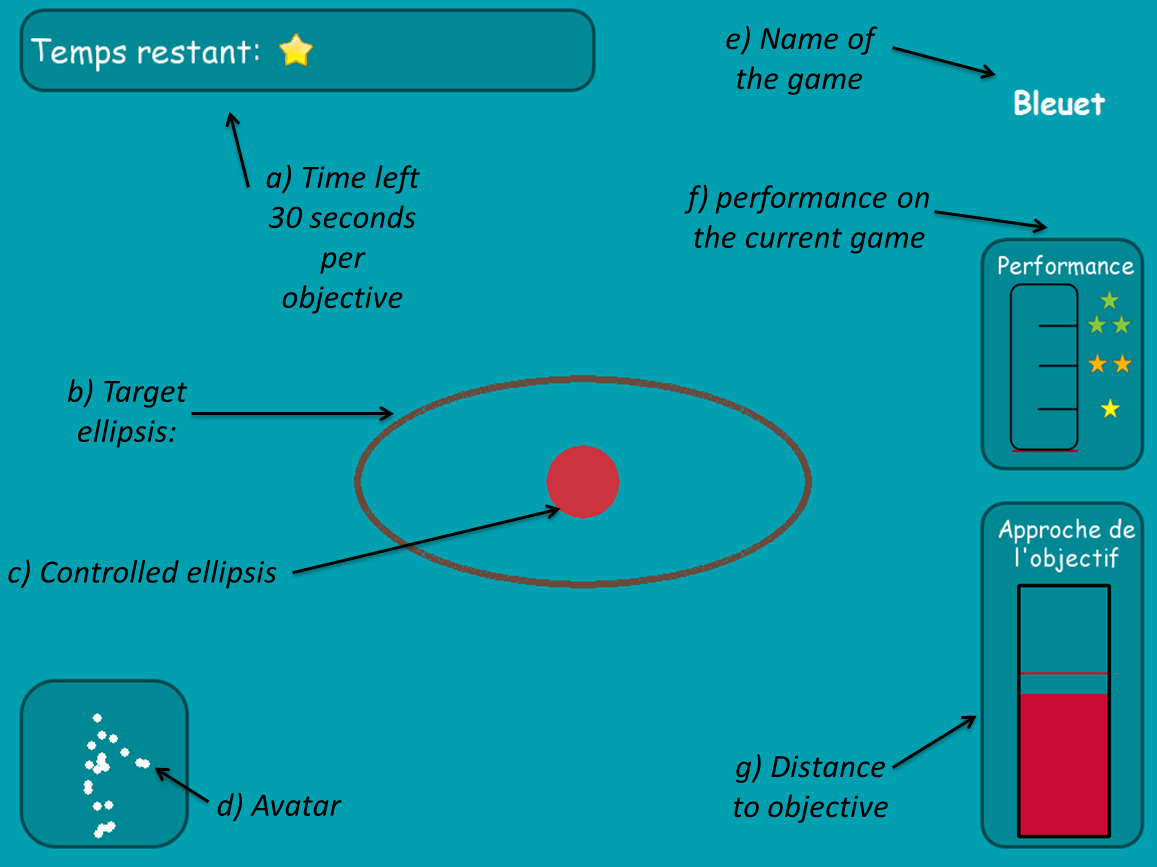
\includegraphics[width=0.9\columnwidth]{images/sc_game_bleuet.PNG}
\end{center}

{\large The game as dipslayed on the screen. The participants have feedback about they performance on the game.}

}

\block{Results and Future work}{
\vspace{1cm}

In our preliminary study, we recorded each time a goal was reached (goal were changing every 30s when not reached), so we could compute the learning progression over a time window, and each time users decided to changed games.

We also recorded the movement of their 20 articulations of their bodies in 3D at 10Hz, the evolution of the 2D shape they had to control and the target shape. Participants also had to fill in personality and usability questionnaires.

\vspace{3cm}


\begin{center}
    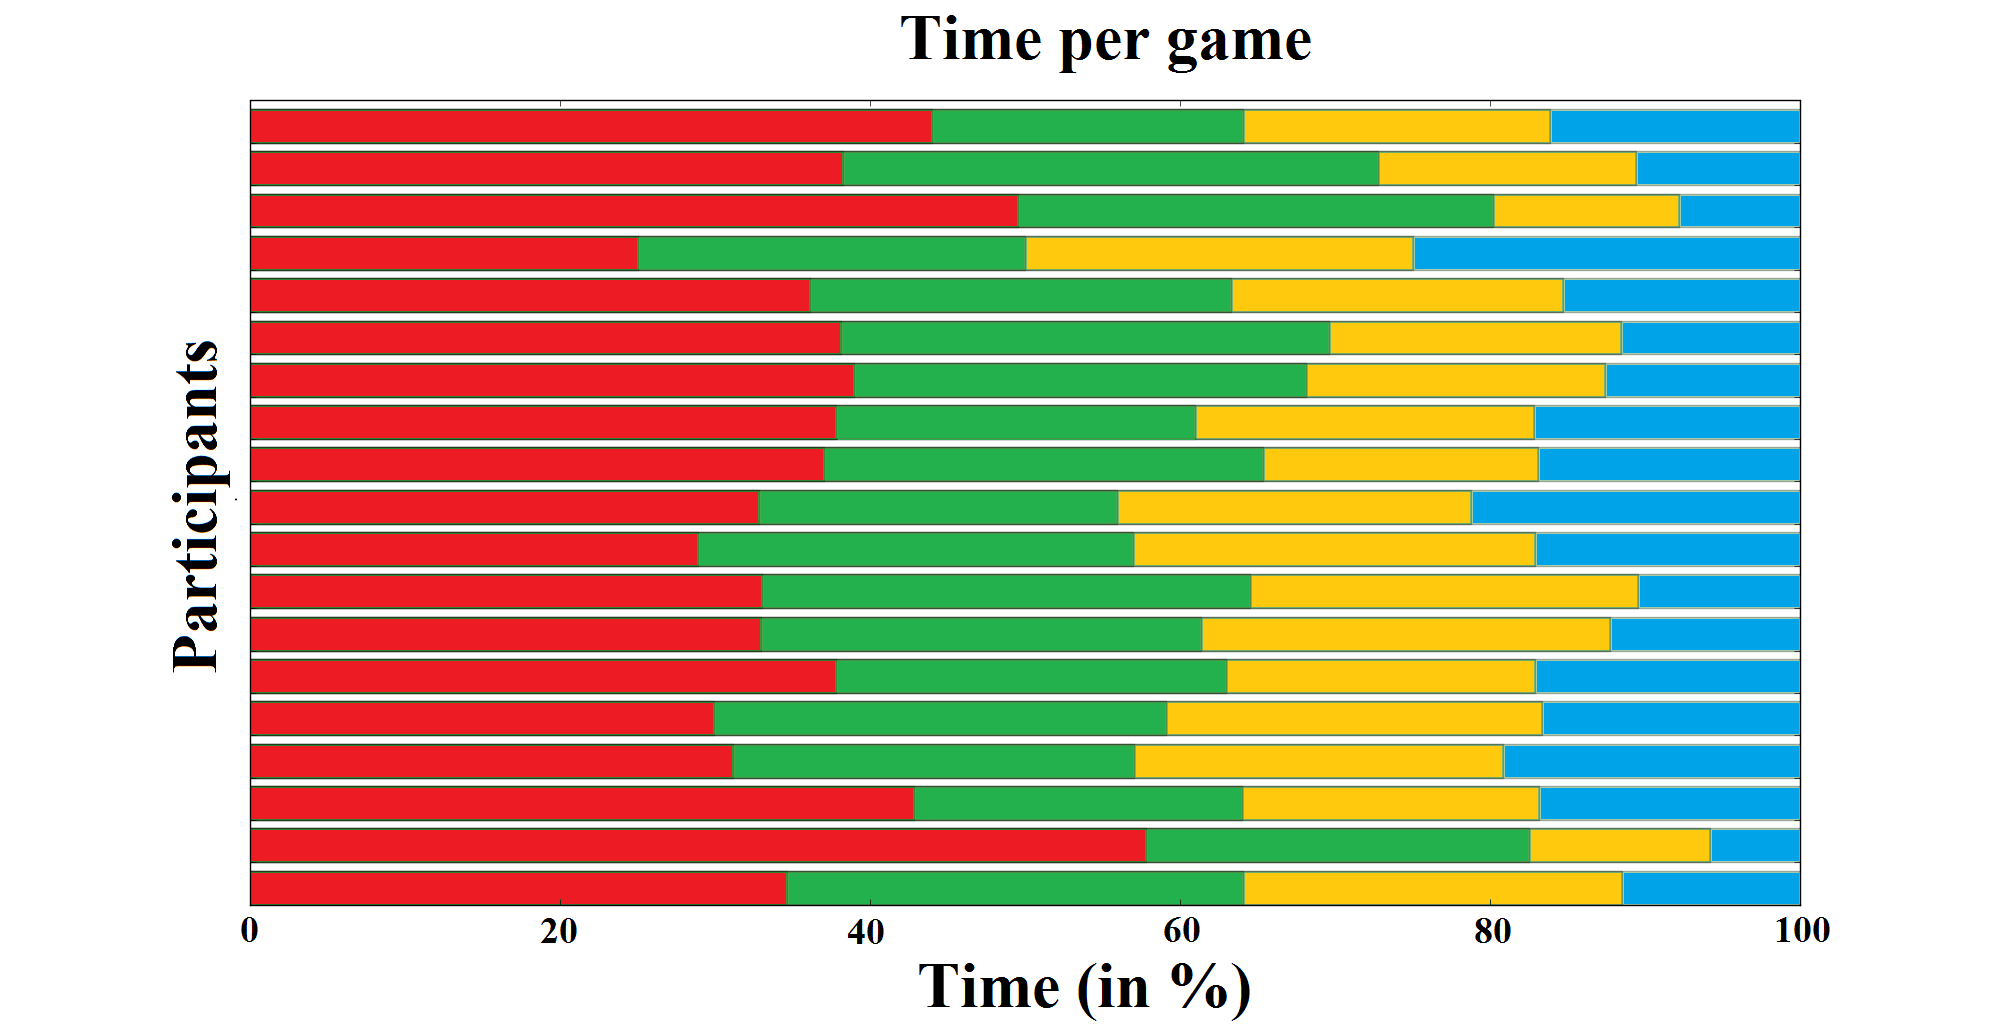
\includegraphics[width=1.0\columnwidth]{images/temps_jeux.png}\\
    {\large Percentage of time spent by subjects on the 4 differents games.}
\end{center}

\vspace{3cm}


We analyzed so far data from 20 participants selected among administrative staffs and students at Inria. We observe a different repartition of the time spent per game.

Our future work will consist of trying to infer the reasons from the when and why the participants change game from the data. We particularly want to investigate whether or not the hyphothesis that activity change is related to learning progress.

\begin{center}
    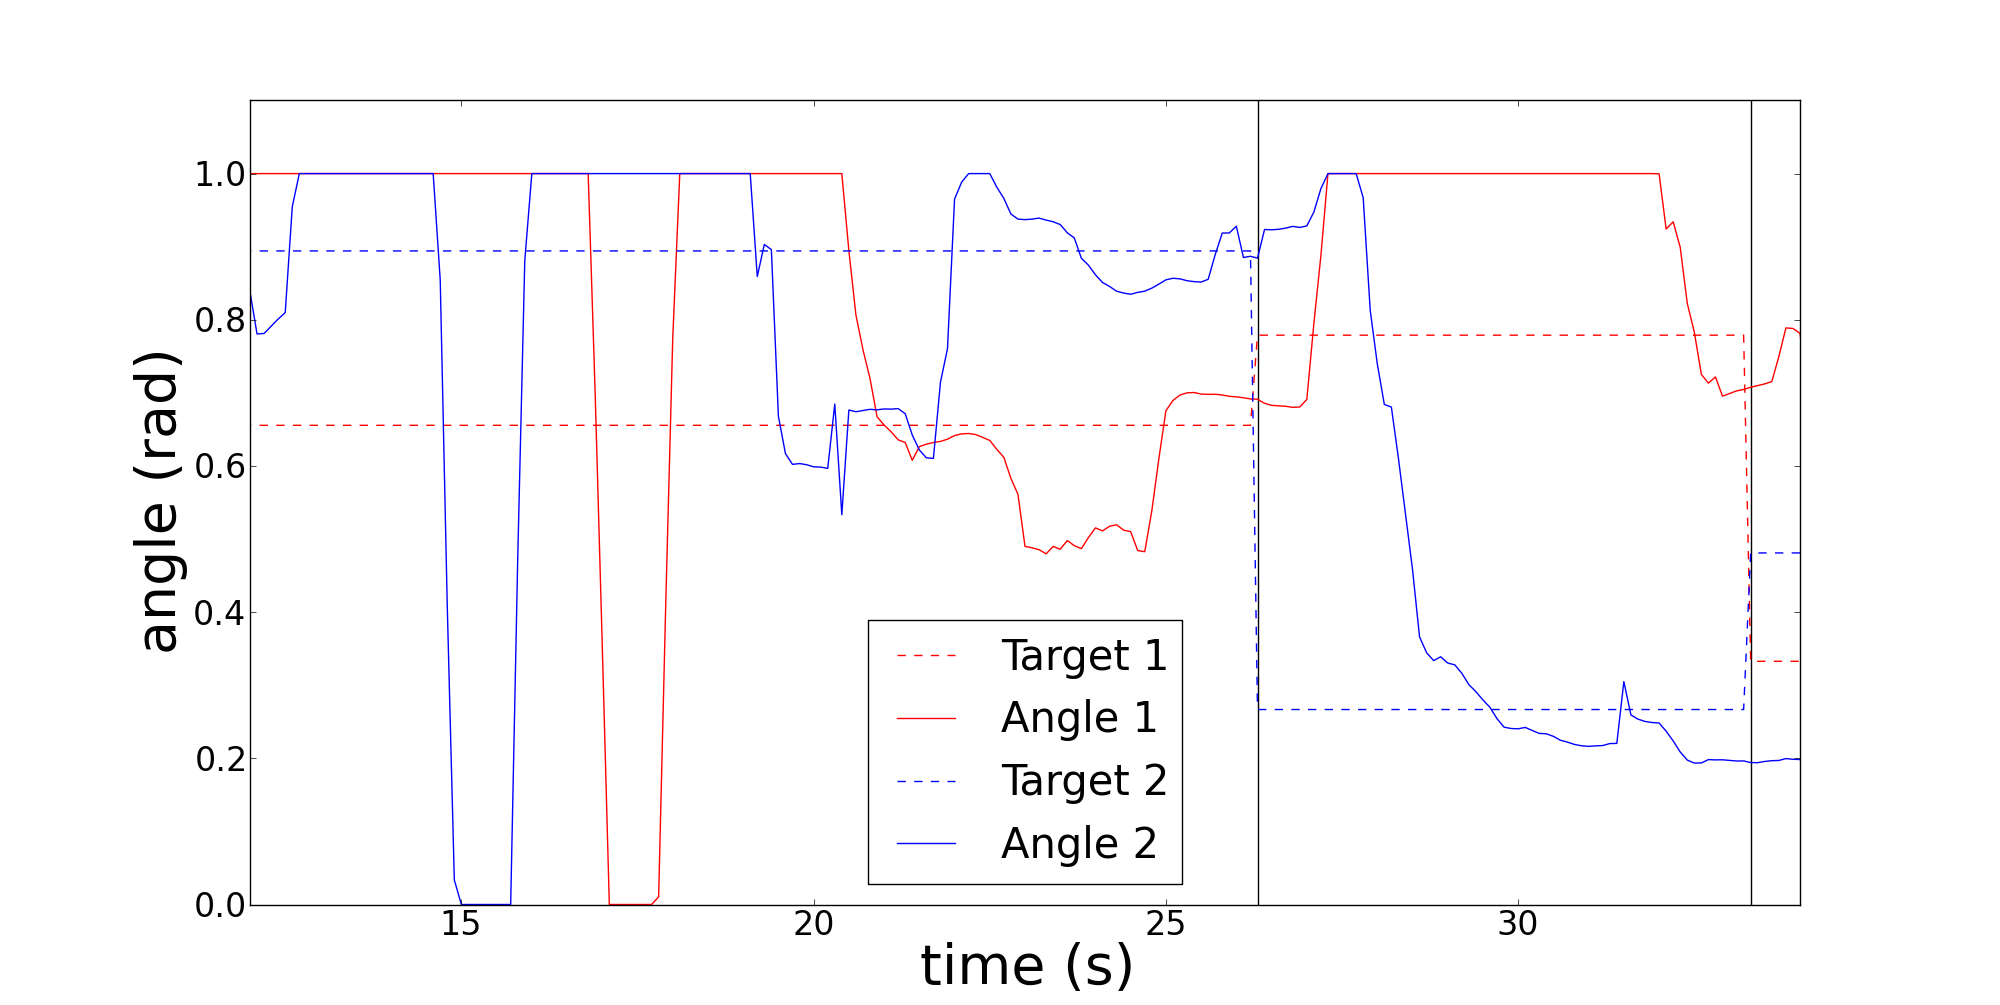
\includegraphics[width=1.0\columnwidth]{images/xp2.png}\\
    {\large We can also analyze the exploratory pattern of each participant.}
\end{center}

\vspace{3cm}

}

\block{References}
{
	% \vspace{-10pt}
	\nocite{*}
	\bibliographystyle{abbrv}
	\renewcommand{\section}[2]{}% Hack to remove bibliography title
	\bibliography{ref}
	\vspace{-10pt}
}

\end{multicols}
\vfill
\end{document}
